\documentclass[14pt]{beamer}
\usepackage{hyperref}
\usepackage{ulem}
\usepackage[T1]{fontenc}
\usetheme{Madrid}

%% Enable license helpers
\graphicspath{ {../cc_beamer/}{pictures/} }
%%%%%%%%%%%%%%%%%%%%%%%%%%%%%%%%%%%%%%%%%%%%%%%%%%%%%%%%%%%%%%%%
%% ccBeamer 0.1, 2007-07-02                                   %%
%% Written by Sebastian Pipping <webmaster@hartwork.org>      %%
%% ---------------------------------------------------------- %%
%% Licensed under Creative Commons Attribution-ShareAlike 3.0 %%
%% http://creativecommons.org/licenses/by-sa/3.0/             %%
%%%%%%%%%%%%%%%%%%%%%%%%%%%%%%%%%%%%%%%%%%%%%%%%%%%%%%%%%%%%%%%%


%% Images
\newcommand{\CcImageBy}[1]{%
	
\includegraphics[scale=#1]{creative_commons/cc_by_30.pdf}%
}
\newcommand{\CcImageCc}[1]{%
	
\includegraphics[scale=#1]{creative_commons/cc_cc_30.pdf}%
}
\newcommand{\CcImageDevNations}[1]{%
	
\includegraphics[scale=#1]{creative_commons/cc_dev_nations_30.pdf}%
}
\newcommand{\CcImageNc}[1]{%
	
\includegraphics[scale=#1]{creative_commons/cc_nc_30.pdf}%
}
\newcommand{\CcImageNd}[1]{%
	
\includegraphics[scale=#1]{creative_commons/cc_nd_30.pdf}%
}
\newcommand{\CcImagePd}[1]{%
	
\includegraphics[scale=#1]{creative_commons/cc_pd_30.pdf}%
}
\newcommand{\CcImageSa}[1]{%
	
\includegraphics[scale=#1]{creative_commons/cc_sa_30.pdf}%
}
\newcommand{\CcImageSampling}[1]{%
	
\includegraphics[scale=#1]{creative_commons/cc_sampling_30.pdf}%
}
\newcommand{\CcImageSamplingPlus}[1]{%
	
\includegraphics[scale=#1]{creative_commons/cc_sampling_plus_30.pdf}%
}


%% Groups
\newcommand{\CcGroupBy}[1]{% zoom
	\CcImageBy{#1}%
}
\newcommand{\CcGroupByNc}[2]{% zoom, gap
	\CcImageBy{#1}\hspace*{#2}\CcImageNc{#1}%
}
\newcommand{\CcGroupByNcNd}[2]{% zoom, gap
	\CcImageBy{#1}\hspace*{#2}\CcImageNc{#1}\hspace*{#2}\CcImageNd{#1}%
}
\newcommand{\CcGroupByNcSa}[2]{% zoom, gap
	\CcImageBy{#1}\hspace*{#2}\CcImageNc{#1}\hspace*{#2}\CcImageSa{#1}%
}
\newcommand{\CcGroupByNd}[2]{% zoom, gap
	\CcImageBy{#1}\hspace*{#2}\CcImageNd{#1}%
}
\newcommand{\CcGroupBySa}[2]{% zoom, gap
	\CcImageBy{#1}\hspace*{#2}\CcImageSa{#1}%
}
\newcommand{\CcGroupDevNations}[1]{% zoom
	\CcImageDevNations{#1}%
}
\newcommand{\CcGroupNcSampling}[2]{% zoom, gap
	\CcImageNc{#1}\hspace*{#2}\CcImageSampling{#1}%
}
\newcommand{\CcGroupPd}[1]{% zoom
	\CcImagePd{#1}%
}
\newcommand{\CcGroupSampling}[1]{% zoom
	\CcImageSampling{#1}%
}
\newcommand{\CcGroupSamplingPlus}[1]{% zoom
	\CcImageSamplingPlus{#1}%
}


%% Text
\newcommand{\CcLongnameBy}{Attribution}
\newcommand{\CcLongnameByNc}{Attribution-NonCommercial}
\newcommand{\CcLongnameByNcNd}{Attribution-NoDerivs}
\newcommand{\CcLongnameByNcSa}{Attribution-NonCommercial-ShareAlike}
\newcommand{\CcLongnameByNd}{Attribution-NoDerivs}
\newcommand{\CcLongnameBySa}{Attribution-ShareAlike}

\newcommand{\CcNote}[1]{% longname
	This work is licensed under the \textit{Creative Commons #1 3.0 License}.%
}


\title[365 days of Open Source]{What I learned from 365 days of contributing to Open Source projects}
\author{Dieter Adriaenssens}
\institute[]{Open Source developer - @dcadriaenssens}
\date[DebConf16 3Jul2016]{DebConf 2016 - Cape Town, South Africa\\
July 3rd, 2016}
\subject{365 days of Open Source}
\begin{document}
  \begin{frame}
    \titlepage
    \vfill
    \begin{center}
      \CcGroupByNcSa{0.83}{0.95ex}\\[2.5ex]
        {\tiny\CcNote{\CcLongnameByNcSa}}
        \vspace*{-2.5ex}
    \end{center}
  \end{frame}
  \begin{frame}
    \frametitle{Introduction}
    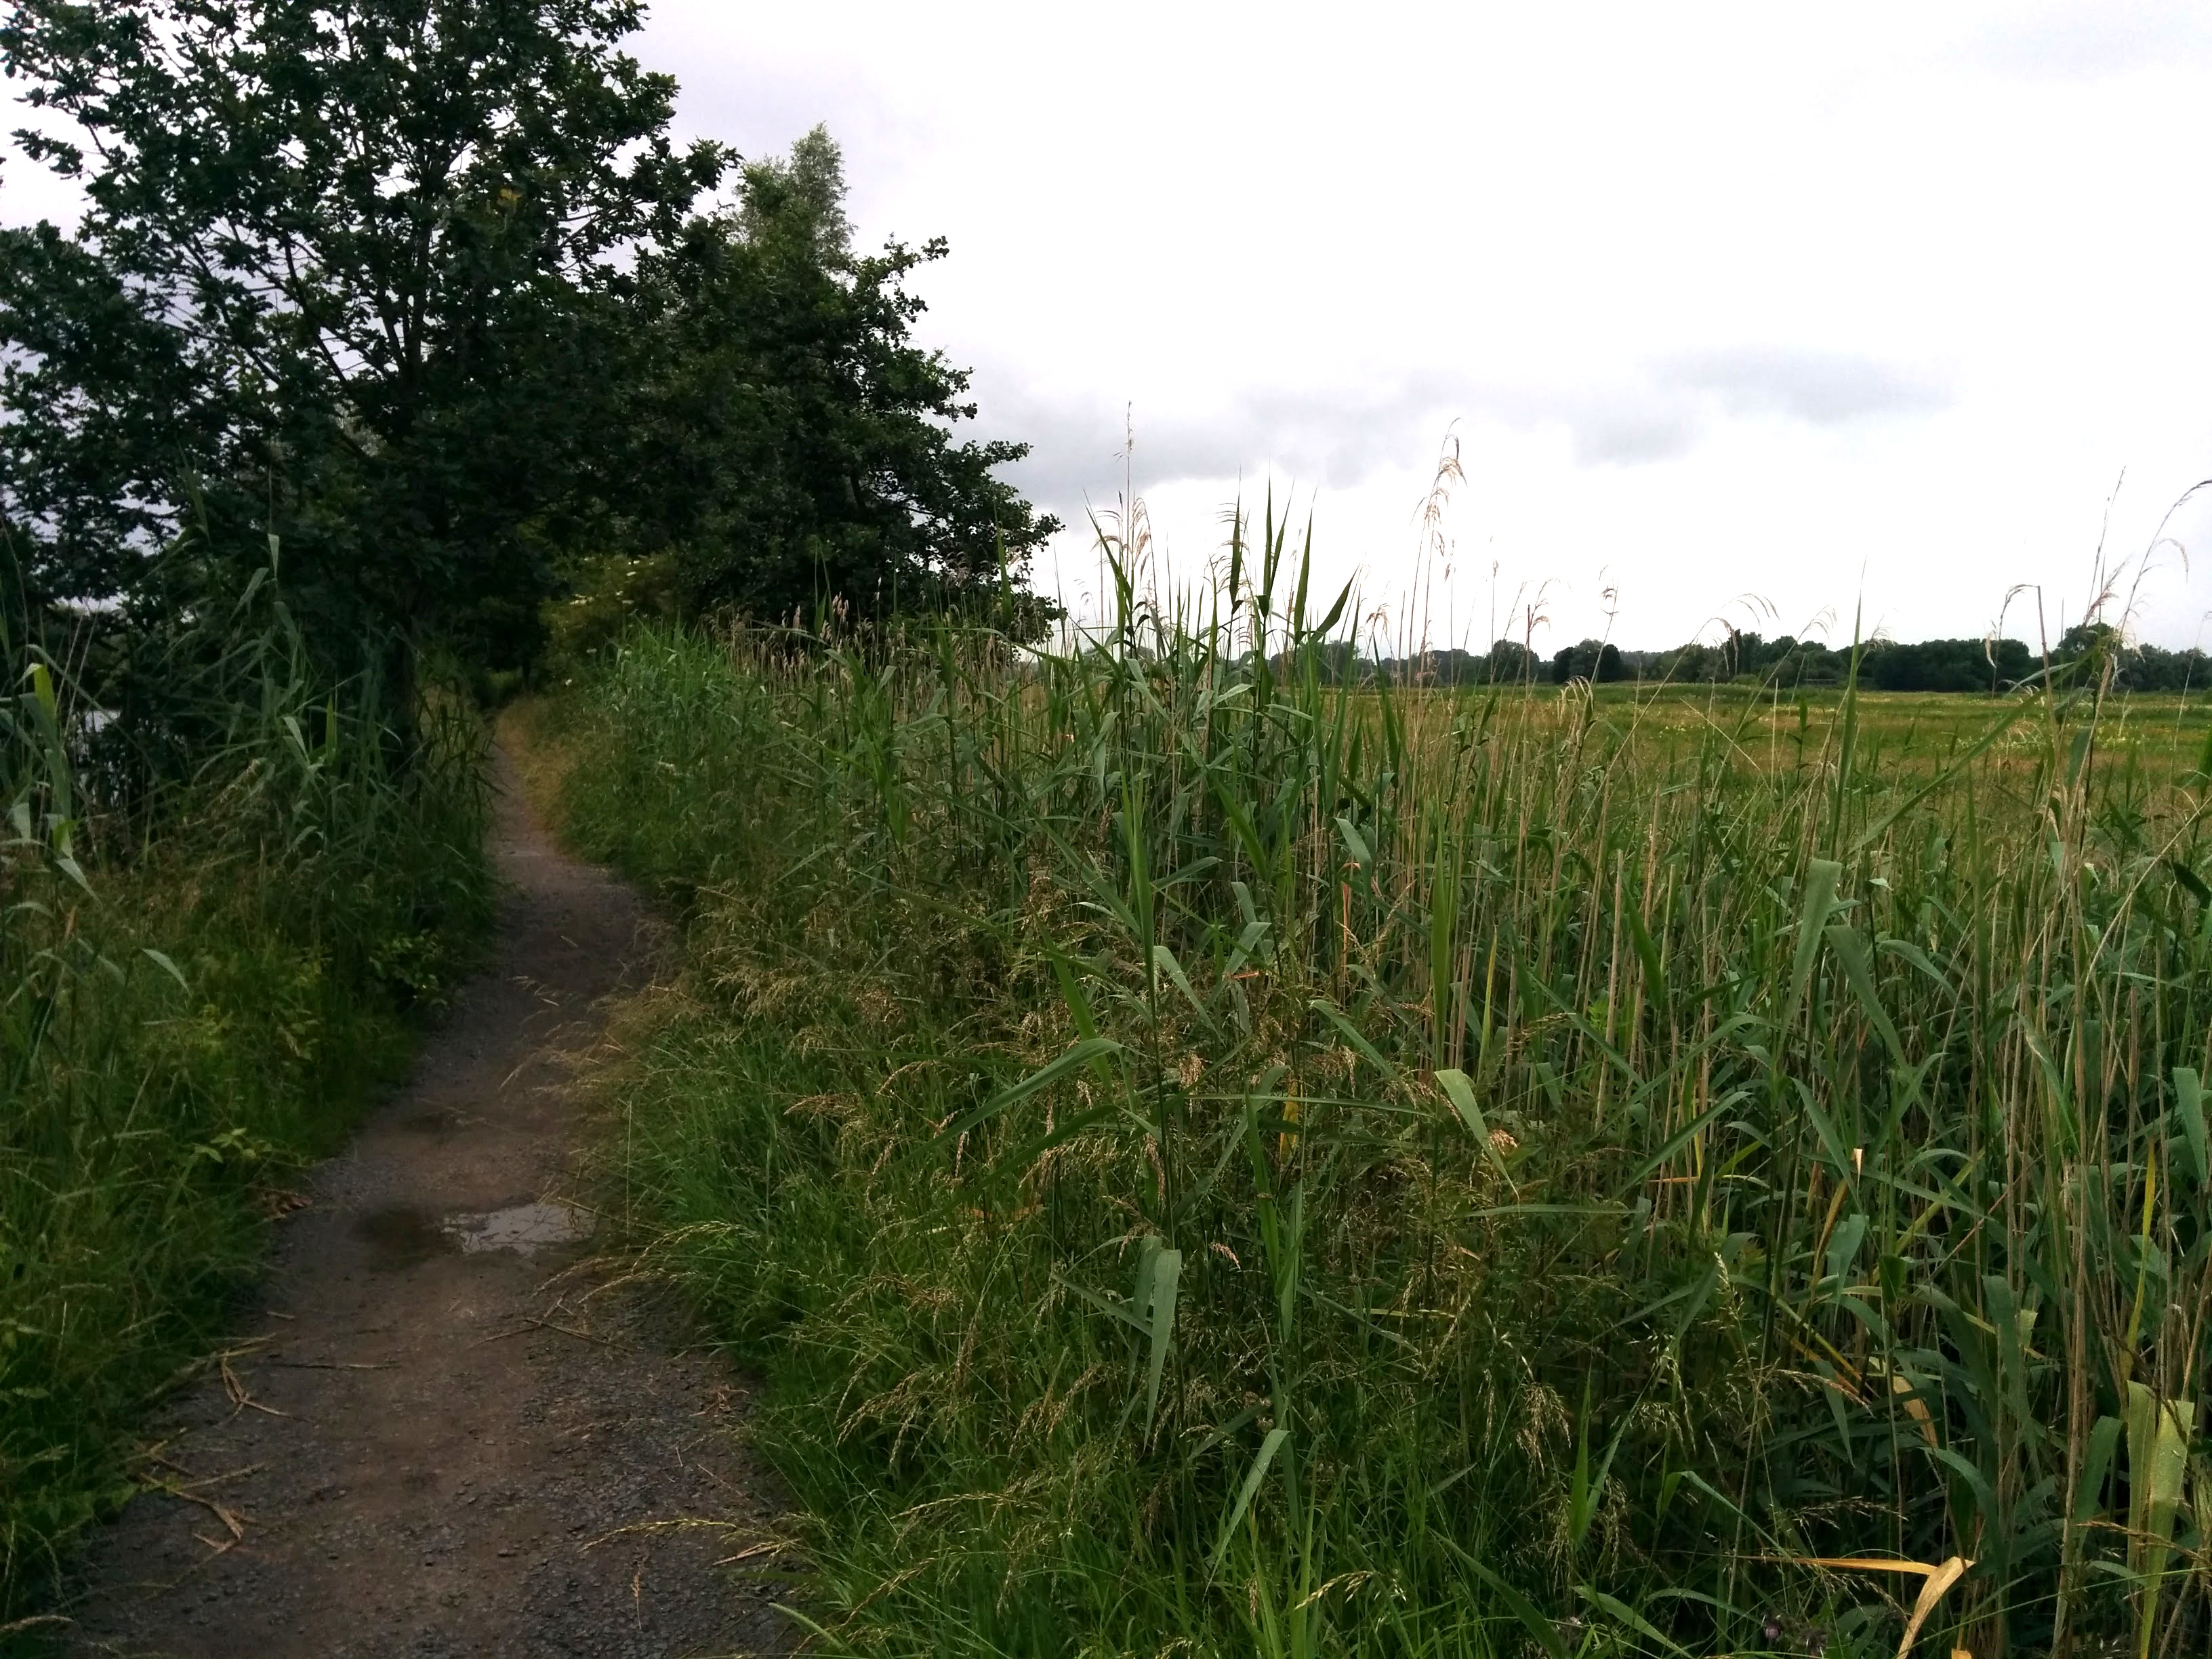
\includegraphics[scale=.1]{Bourgoyen.jpg}
  \end{frame}
  \begin{frame}
    \frametitle{Introduction}
    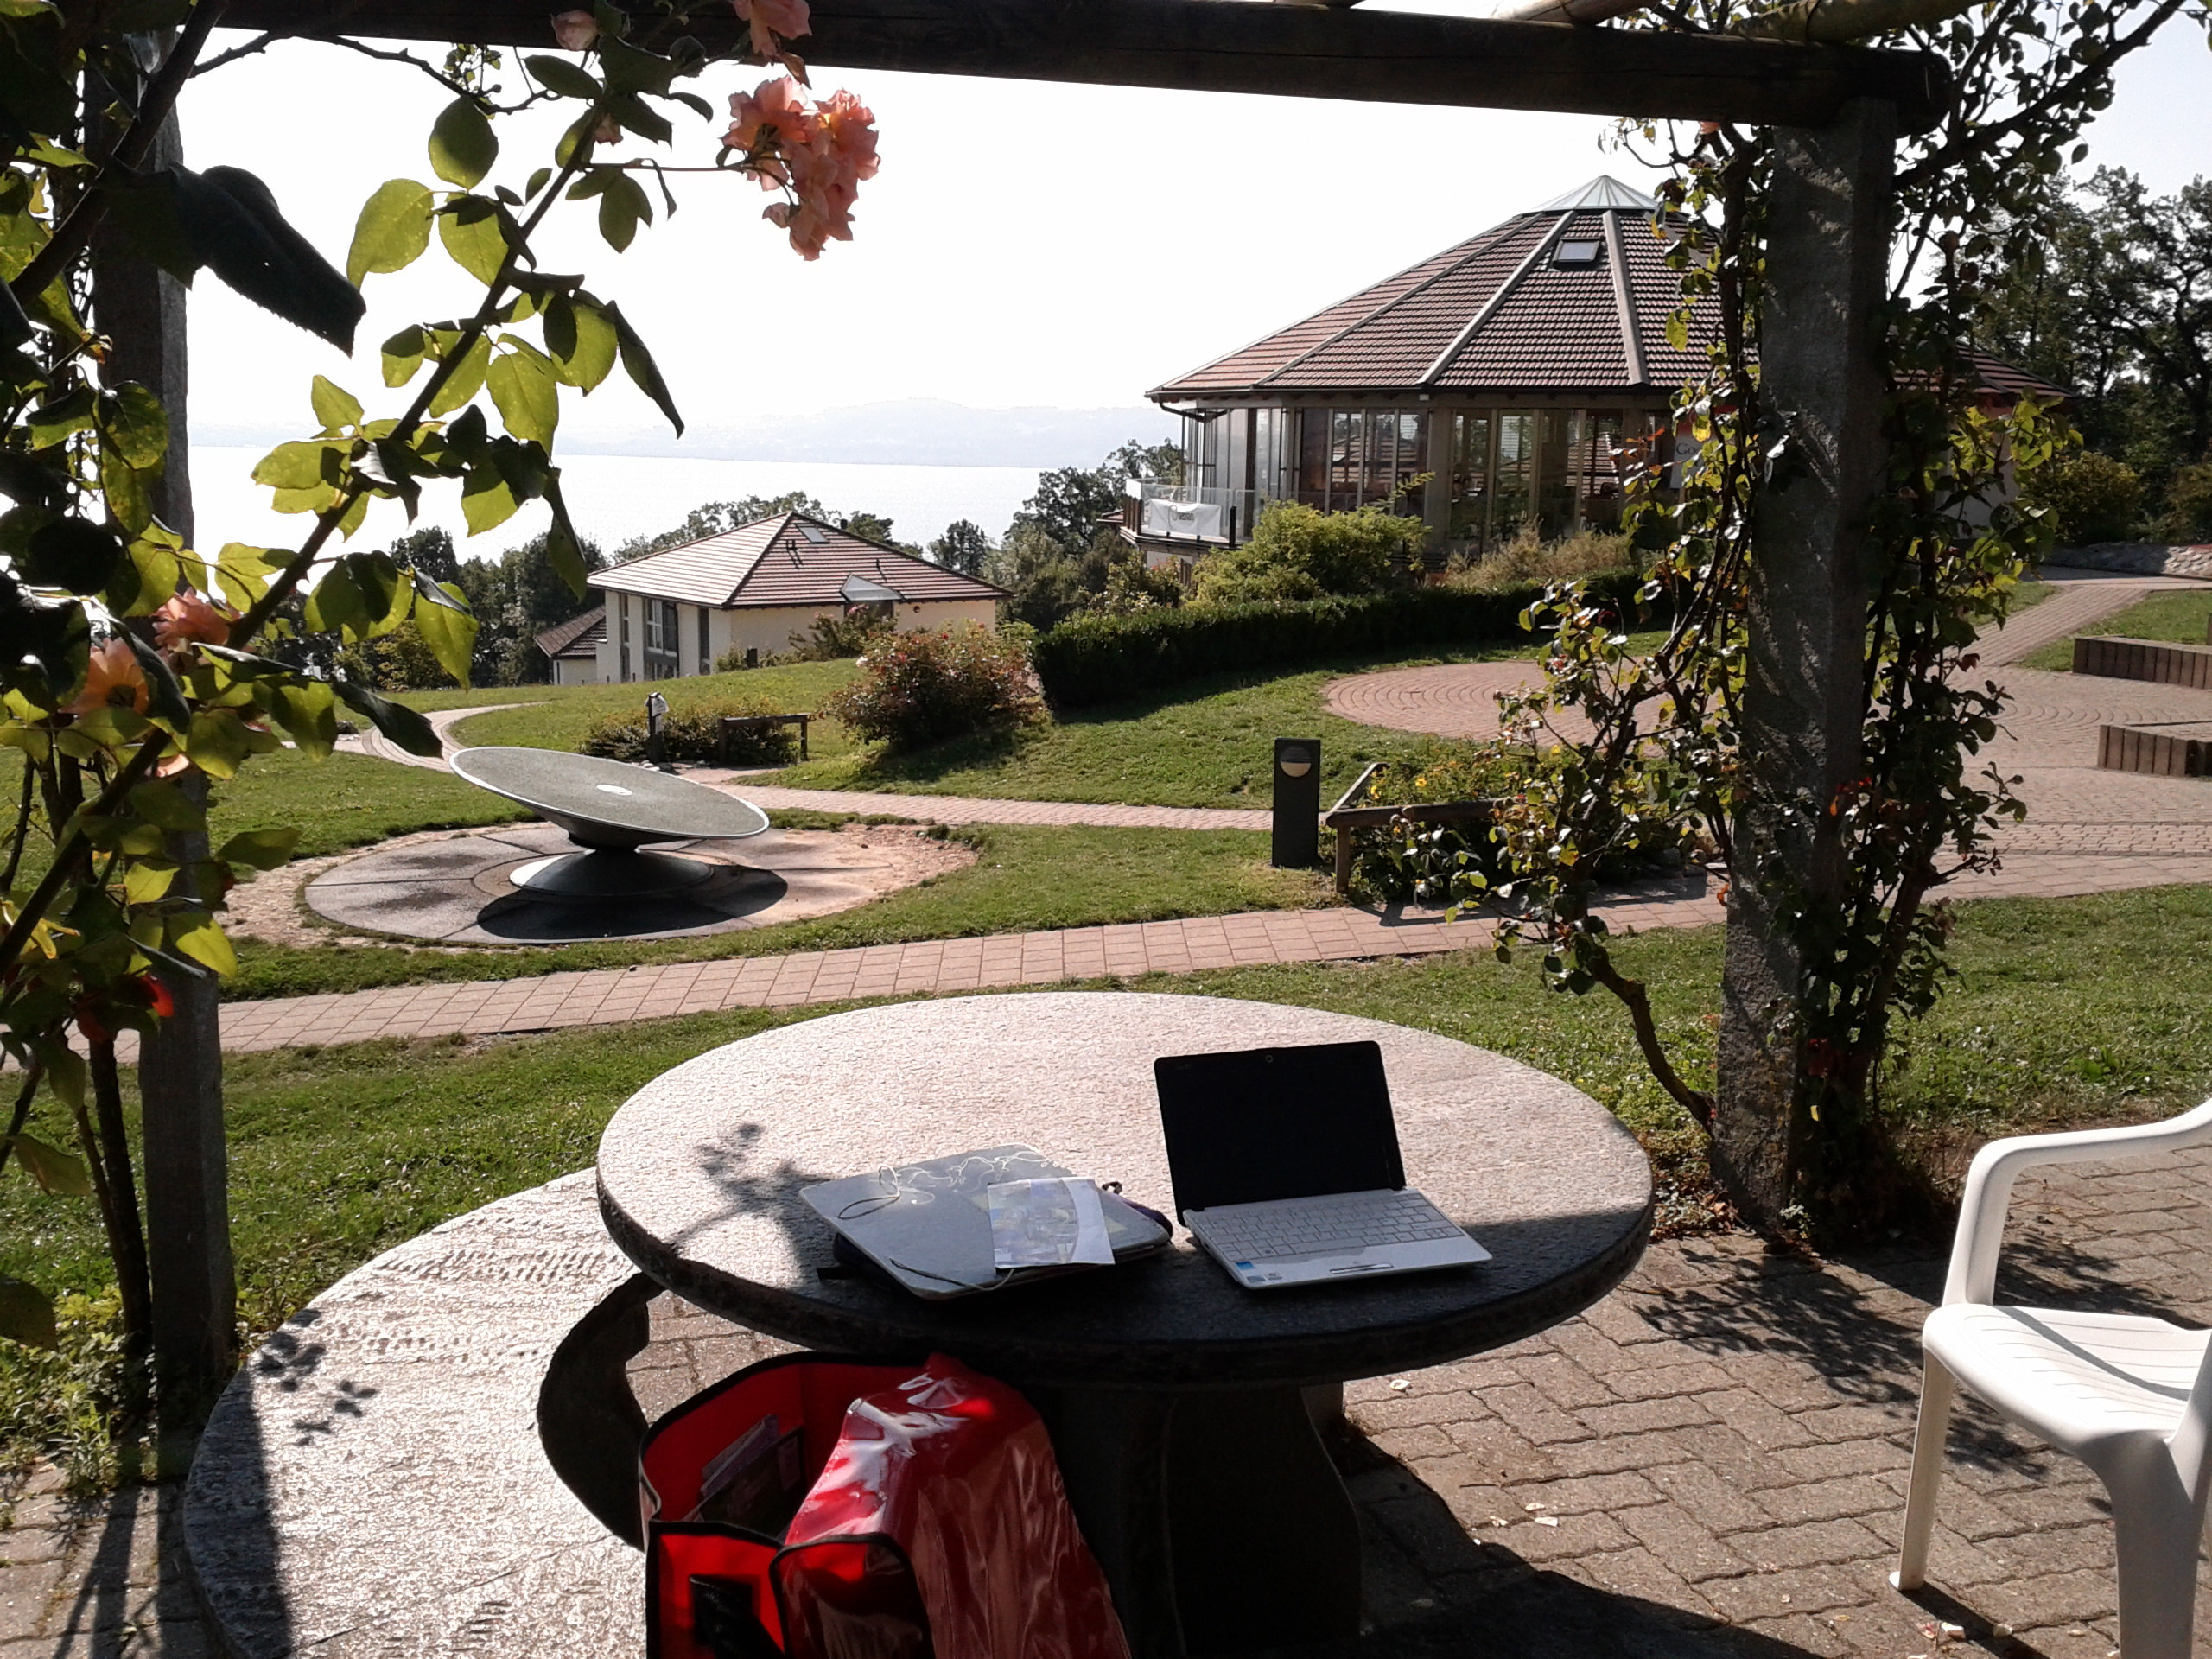
\includegraphics[scale=.125]{DebConf2013.jpg}
  \end{frame}
  \begin{frame}
    \frametitle{Introduction}
    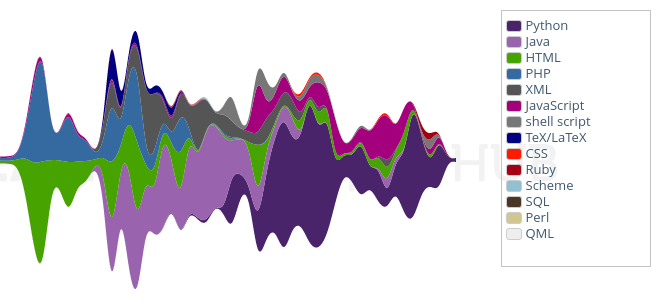
\includegraphics[scale=.3]{openhub.png}
    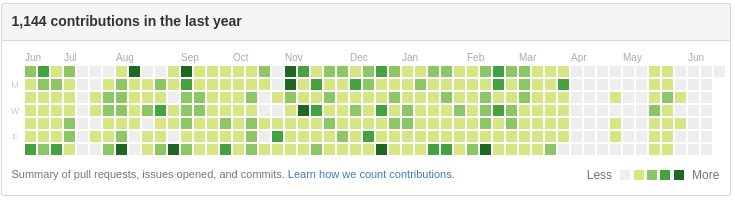
\includegraphics[scale=.3]{github_19jun2016.png}\\
    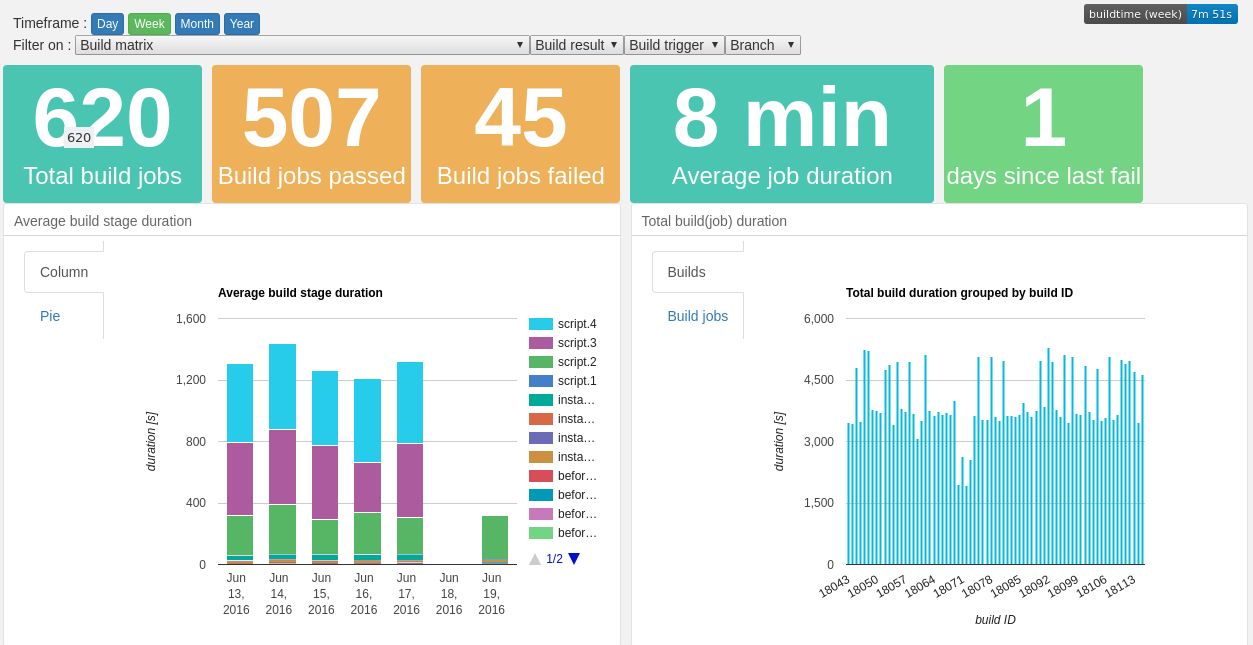
\includegraphics[scale=.3]{screenshot_buildtimetrend.png}
  \end{frame}
  \begin{frame}
    \frametitle{How it started}
    \begin{itemize}
      \item 14 January 2014 : I returned from an 'unplugged' holiday
      \item previous 100+ day commit streaks
      \item see how far I would get
    \end{itemize}
  \end{frame}
  \begin{frame}
    \frametitle{What and how}
    \begin{itemize}
      \item at least 1 commit per day
      \item Open Source projects hosted on Github (public repos)
      \item any type of contribution
      \item after day-job
    \end{itemize}
  \end{frame}
  \begin{frame}
    \frametitle{Planning}
    \begin{itemize}
      \item larger tasks :
      \begin{itemize}
        \item new features
        \item bug fixes
        \item refactoring
        \item unit tests
      \end{itemize}
      \item availability of :
      \begin{itemize}
        \item time
        \item internet
        \item infrastructure
      \end{itemize}
    \end{itemize}
  \end{frame}
  \begin{frame}
    \frametitle{Planning}
    \begin{itemize}
      \item keep a list of smaller/easier tasks :
      \begin{itemize}
        \item fix coding style
        \item fix typos
        \item translations
      \end{itemize}
      \item for emergencies ;)
      \item code quality improves
      \item one commit leads to another
    \end{itemize}
  \end{frame}
  \begin{frame}
    \frametitle{June 2014 : Getting serious}
    \begin{itemize}
      \item Josh (@dzello), Open Sourcerer at Keen.io pledged to do a 365 day commit streak
      \item I was at 162 days
      \item I took the challenge to do a 365 day streak
    \end{itemize}
  \end{frame}
  \begin{frame}
    \frametitle{Holiday}
    \begin{columns}
      \begin{column}{0.5\textwidth}
        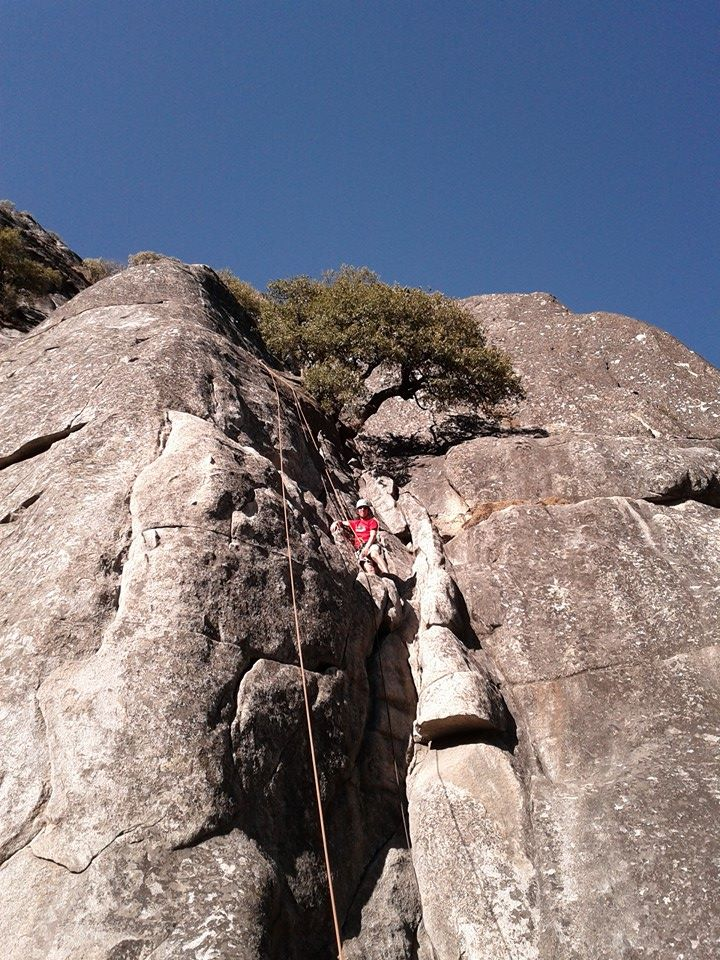
\includegraphics[scale=.25]{climbing.jpg}
      \end{column}
      \begin{column}{0.5\textwidth}
        \begin{itemize}
          \item July 2014 : climbing trip
          \item climbing during the day
          \item limited time in the evening
          \item planning to do small commits
          \item close call on a few days
        \end{itemize}
      \end{column}
    \end{columns}
  \end{frame}
  \begin{frame}
    \frametitle{Difficulties}
    Can I keep the streak going?
    \begin{itemize}
      \item busy day at work
      \item other things to do (friends, family, sports, \ldots)
      \item stuck on a problem
      \item traveling
      \item timezones
    \end{itemize}
  \end{frame}
  \begin{frame}
    \frametitle{Tips}
    \begin{itemize}
      \item easy tasks list
      \item commit time
      \item commit just before/after midnight
      \item issues and pull requests
    \end{itemize}
  \end{frame}
  \begin{frame}
    \frametitle{Meeting Josh in San Francisco (Oct 2014)}
    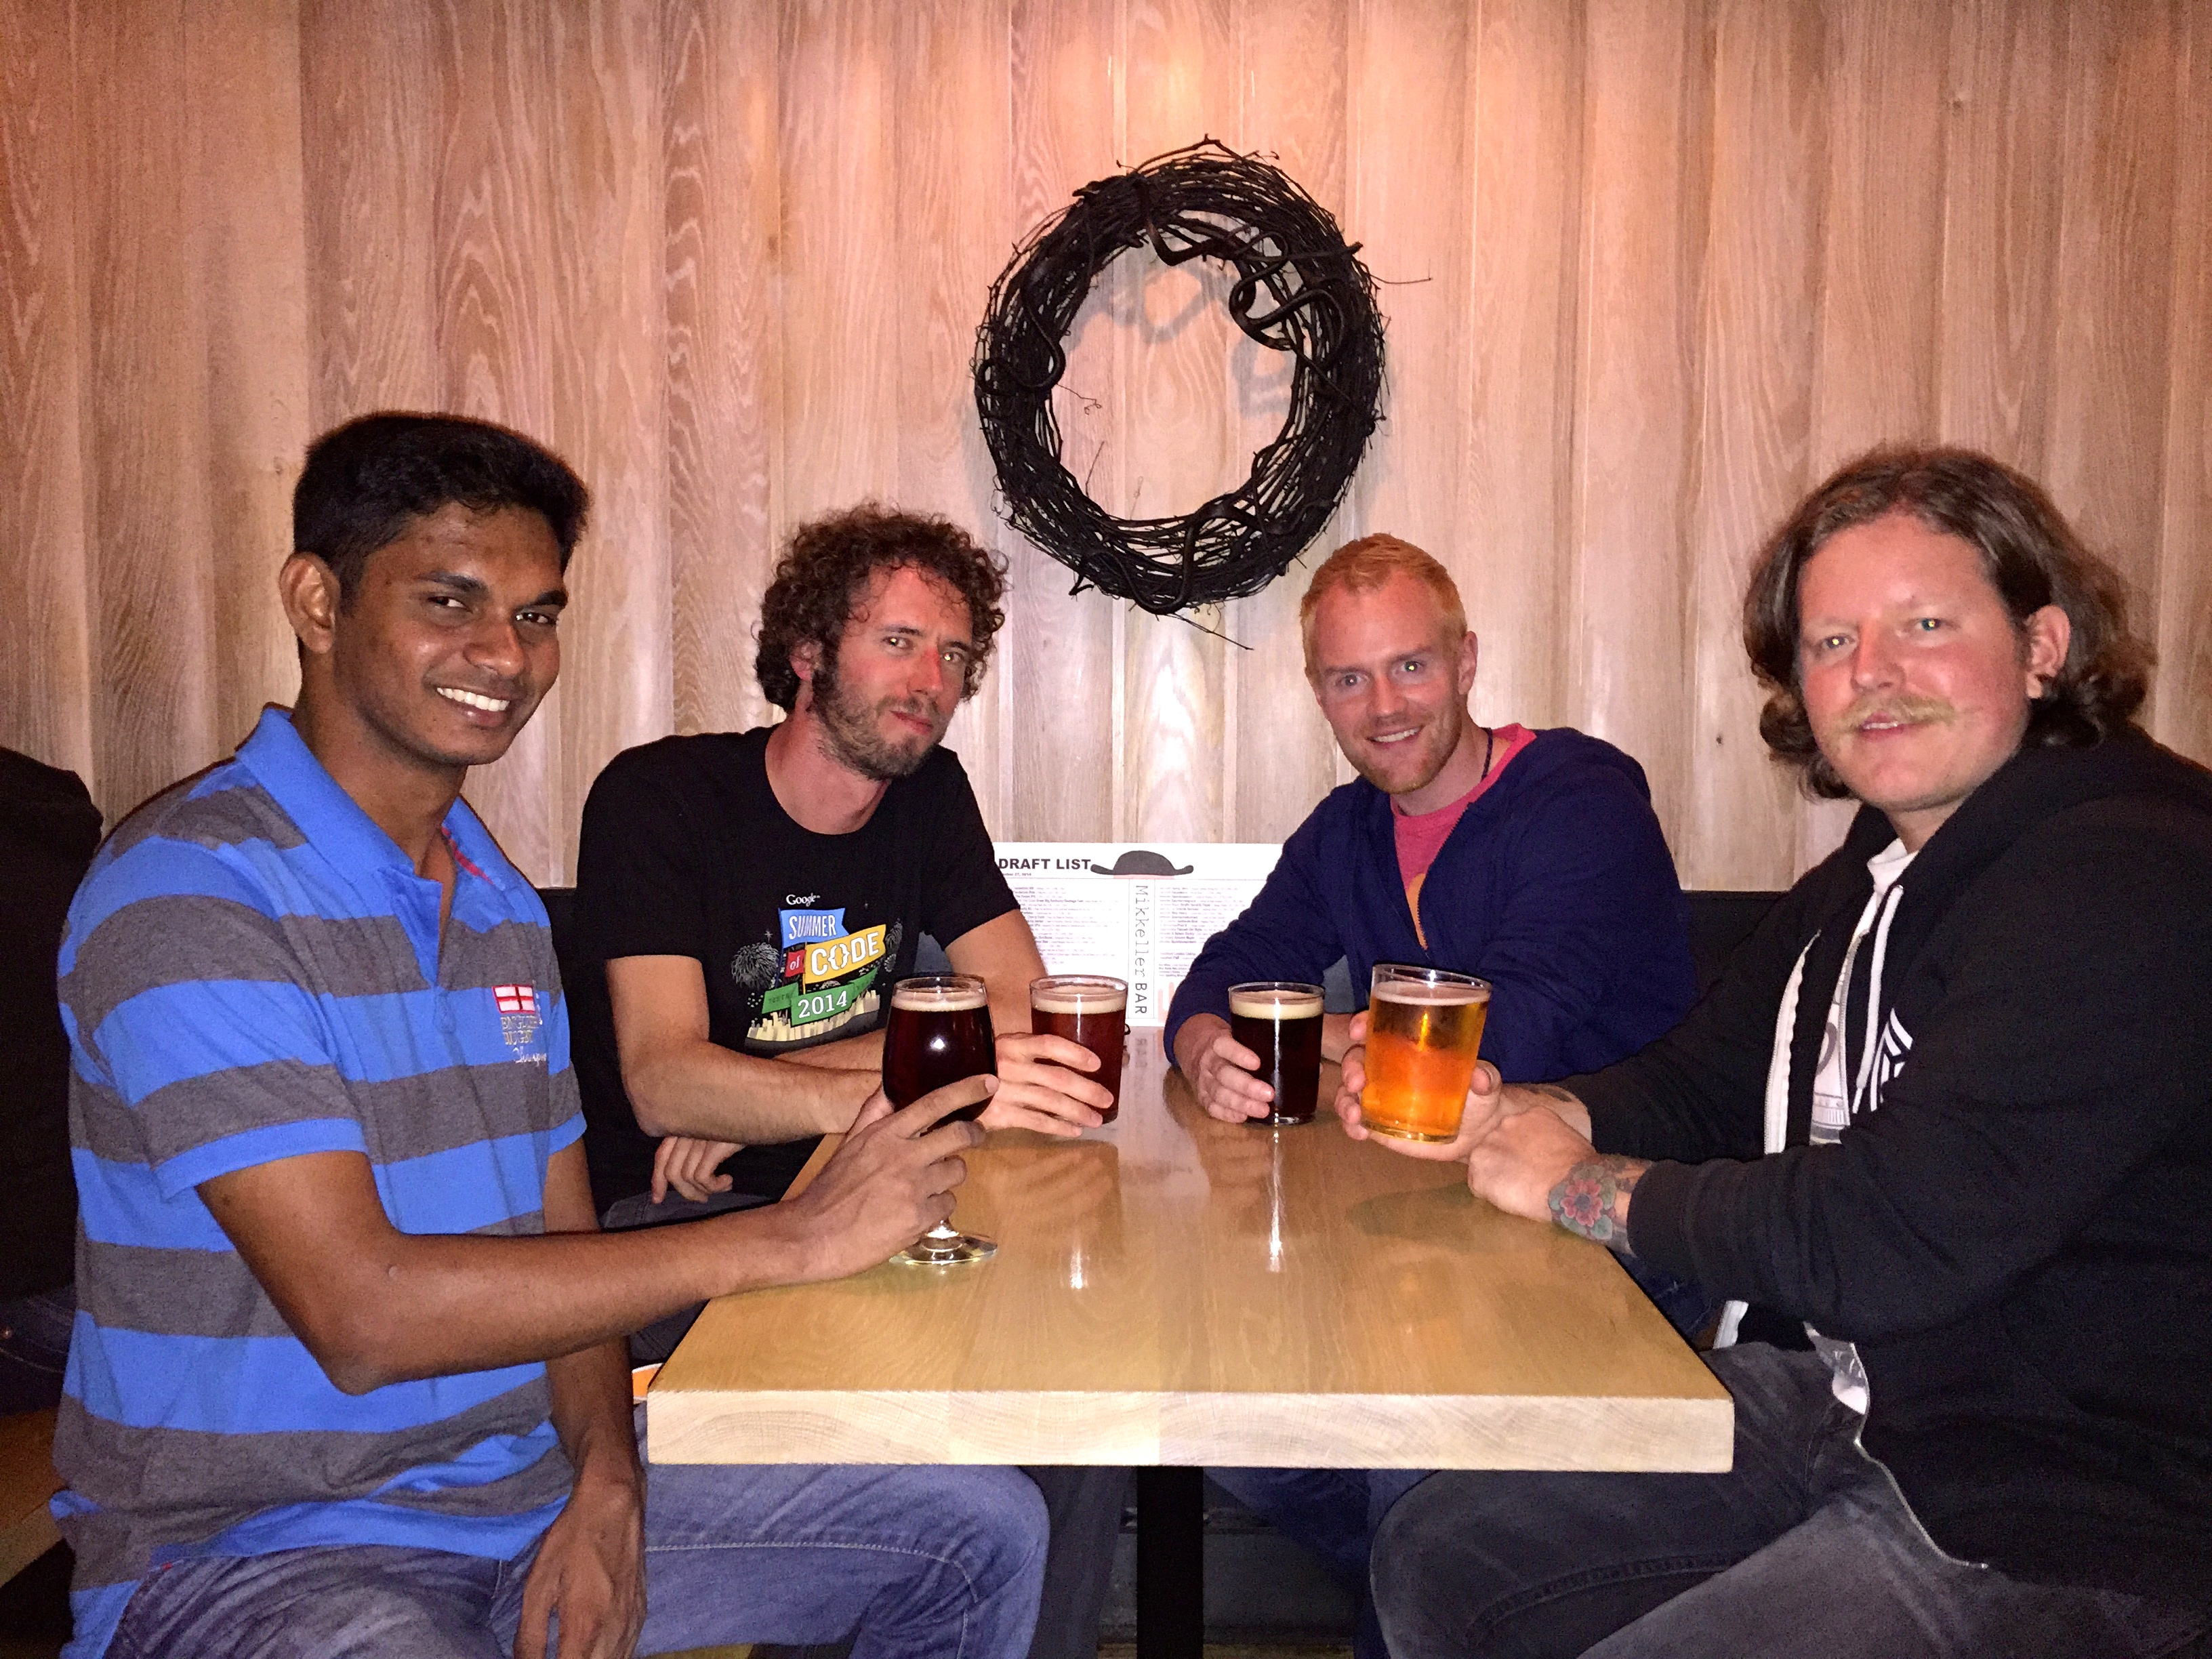
\includegraphics[scale=.1]{josh_justin.jpg}
  \end{frame}
  \begin{frame}
    \frametitle{Josh's experience}
    \begin{itemize}
      \item Josh stopped his 66 day streak going to Burning Man
      \item different ways of measuring progress
      \item other people with a considerable streak : relieved it was over
    \end{itemize}
  \end{frame}
  \begin{frame}
    \frametitle{365 days of Open Source}
    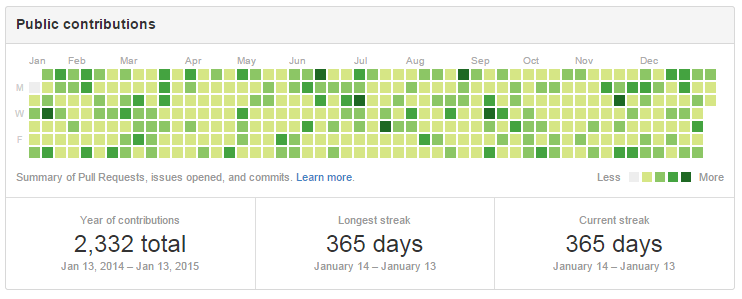
\includegraphics[scale=.45]{github_oss365_13jan2015.png}
    \begin{itemize}
      \item 13Jan2015 : 365 day commit streak!
      \item 10Apr2015 : End of commit streak after 452 days
    \end{itemize}
  \end{frame}
  \begin{frame}
    \frametitle{Cheating}
    \begin{itemize}
      \item bogus commit
      \item cronjob
      \item change commit time
    \end{itemize}
    Value of a streak?
  \end{frame}
  \begin{frame}
    \frametitle{Lessons learned}
    \begin{itemize}
      \item set a realistic goal
      \item choose something that works for you
      \item 1 commit per day creates a habbit
      \item warning : afraid to break the streak
    \end{itemize}
  \end{frame}
  \begin{frame}
    \frametitle{Lessons learned}
    \begin{itemize}
      \item contributing to a project should be the primary drive
      \item metrics are just a means
      \item don't let the metrics drive you
      \item similarities in sports, goals, projects, \ldots
      \item find a balance between work and relaxing : take regular breaks
    \end{itemize}
  \end{frame}
  \begin{frame}
    \frametitle{Acknowledgements}
    Big thanks to input from
    \begin{itemize}
      \item Josh Dzielak (\href{https://twitter.com/dzello}{@dzello})
      \item \href{https://twitter.com/ryanseys}{@ryanseys}
      \item \href{https://twitter.com/natashatherobot}{@NatashaTheRobot}
      \item \href{https://twitter.com/gjermundbjaanes}{@gjermundbjaanes}
      \item Erik Romijn (\href{https://twitter.com/erikpub}{@erikpub})
    \end{itemize}
  \end{frame}
  \begin{frame}
   \frametitle{Questions?}
    Dieter Adriaenssens - \href{https://twitter.com/dcadriaenssens}{\small{@dcadriaenssens}}
    \vfill
    Blogpost : \href{http://ruleant.blogspot.be/2015/01/what-i-learned-from-365-days-of.html}{http://ruleant.blogspot.be/2015/01/what-i-learned-from-365-days-of.html}
  \end{frame}
\end{document}
